\documentclass[border={0.5cm 1cm 0.5cm 1cm}]{standalone}  %E,S,W,N

\usepackage{amssymb}
\usepackage{amsmath}
\usepackage{tikz}
\usetikzlibrary{decorations.pathmorphing}			%for random lines

%from Deleuze - Foucault (1988), p. 120

\begin{document}
	
	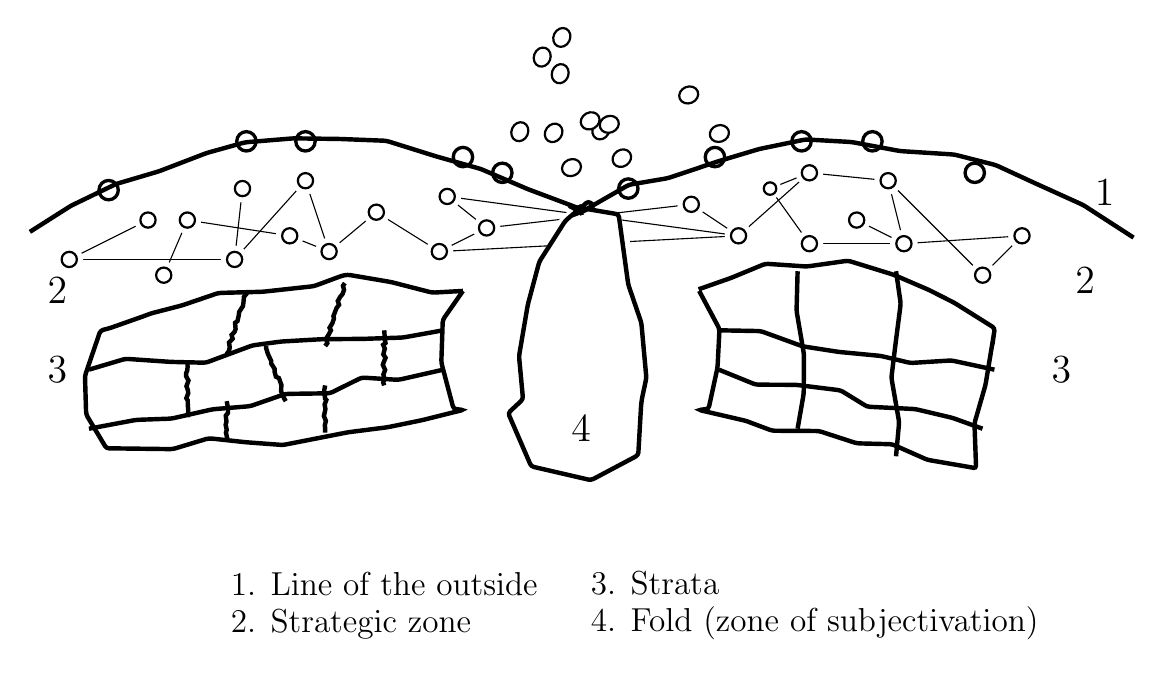
\begin{tikzpicture}
	%DOTS ON ARCS
	\filldraw[fill=white,very thick] (-6,0.28) circle (3.5pt);	%leftmost
	\filldraw[fill=white,very thick] (-4.25,0.9) circle (3.5pt);
	\filldraw[fill=white,very thick] (-3.5,0.9) circle (3.5pt);
	\filldraw[fill=white,very thick] (-1.5,0.7) circle (3.5pt);
	\filldraw[fill=white,very thick] (-1,0.5) circle (3.5pt);
	%
	\filldraw[fill=white,very thick] (0.6,0.3) circle (3.5pt);
	\filldraw[fill=white,very thick] (1.7,0.7) circle (3.5pt);
	\filldraw[fill=white,very thick] (2.8,0.9) circle (3.5pt);
	\filldraw[fill=white,very thick] (3.7,0.9) circle (3.5pt);
	\filldraw[fill=white,very thick] (5,0.5) circle (3.5pt);	%rightmost
	
	%CENTER LINES
	%LEFT
	\draw (-6.5,-0.6)--(-5.5,-0.1);	\draw (-6.5,-0.6)--(-4.4,-0.6);	\draw (-5.3,-0.8)--(-5.0,-0.1);
	\draw (-5.0,-0.1)--(-3.7,-0.3);	\draw (-4.4,-0.6)--(-4.3, 0.3);	\draw (-4.4,-0.6)--(-3.5, 0.4);
	\draw (-3.7,-0.3)--(-3.2,-0.5);	\draw (-3.2,-0.5)--(-3.5, 0.4);	\draw (-3.2,-0.5)--(-2.6, 0.0);
	\draw (-2.6, 0.0)--(-1.8,-0.5);	\draw (-1.8,-0.5)--(-1.2,-0.2);	\draw (-1.2,-0.2)--(-1.7, 0.2);
	%
	%CONNECTING
	\draw (1.4, 0.1)--(-1.2,-0.2);	\draw (2.0,-0.3)--(-1.7, 0.2);	\draw (2.0,-0.3)--(-1.8,-0.5);
	%
	%RIGHT
	\draw (2.0,-0.3)--(1.4, 0.1);	\draw (2.9, 0.5)--(2.0,-0.3);	\draw (2.9, 0.5)--(2.4, 0.3);
	\draw (2.4, 0.3)--(2.9,-0.4);	\draw (3.9, 0.4)--(2.9, 0.5);	\draw (4.1,-0.4)--(2.9,-0.4);
	\draw (4.1,-0.4)--(3.5,-0.1);	\draw (4.1,-0.4)--(3.9, 0.4);	\draw (5.1,-0.8)--(3.9, 0.4);
	\draw (5.6,-0.3)--(4.1,-0.4);	\draw (5.6,-0.3)--(5.1,-0.8);
	
	%CENTER DOTS - RIGHT
	\fill[white](1.4, 0.1) circle (5pt); \filldraw[thick,fill=white] (1.4, 0.1) circle (2.75pt);
	\fill[white](2.0,-0.3) circle (5pt); \filldraw[thick,fill=white] (2.0,-0.3) circle (2.75pt);
	\fill[white](2.4, 0.3) circle (4pt); \filldraw[thick,fill=white] (2.4, 0.3) circle (2.25pt);
	\fill[white](2.9, 0.5) circle (5pt); \filldraw[thick,fill=white] (2.9, 0.5) circle (2.75pt);
	\fill[white](2.9,-0.4) circle (5pt); \filldraw[thick,fill=white] (2.9,-0.4) circle (2.75pt);
	\fill[white](3.5,-0.1) circle (5pt); \filldraw[thick,fill=white] (3.5,-0.1) circle (2.75pt);
	\fill[white](3.9, 0.4) circle (5pt); \filldraw[thick,fill=white] (3.9, 0.4) circle (2.75pt);
	\fill[white](4.1,-0.4) circle (5pt); \filldraw[thick,fill=white] (4.1,-0.4) circle (2.75pt);
	\fill[white](5.1,-0.8) circle (5pt); \filldraw[thick,fill=white] (5.1,-0.8) circle (2.75pt);
	\fill[white](5.6,-0.3) circle (5pt); \filldraw[thick,fill=white] (5.6,-0.3) circle (2.75pt);
	
	%CENTER DOTS - LEFT
	\fill[white](-6.5,-.6) circle (5pt); \filldraw[thick,fill=white] (-6.5,-0.6) circle (2.75pt);
	\fill[white](-5.5,-.1) circle (5pt); \filldraw[thick,fill=white] (-5.5,-0.1) circle (2.75pt);
	\fill[white](-5.3,-.8) circle (5pt); \filldraw[thick,fill=white] (-5.3,-0.8) circle (2.75pt);
	\fill[white](-5.0,-.1) circle (5pt); \filldraw[thick,fill=white] (-5.0,-0.1) circle (2.75pt);
	\fill[white](-4.4,-.6) circle (5pt); \filldraw[thick,fill=white] (-4.4,-0.6) circle (2.75pt);
	\fill[white](-4.3, .3) circle (5pt); \filldraw[thick,fill=white] (-4.3, 0.3) circle (2.75pt);
	\fill[white](-3.5, .4) circle (5pt); \filldraw[thick,fill=white] (-3.5, 0.4) circle (2.75pt);
	\fill[white](-3.7,-.3) circle (5pt); \filldraw[thick,fill=white] (-3.7,-0.3) circle (2.75pt);
	\fill[white](-3.2,-.5) circle (5pt); \filldraw[thick,fill=white] (-3.2,-0.5) circle (2.75pt);
	\fill[white](-2.6, .0) circle (5pt); \filldraw[thick,fill=white] (-2.6, 0.0) circle (2.75pt);
	\fill[white](-1.8,-.5) circle (5pt); \filldraw[thick,fill=white] (-1.8,-0.5) circle (2.75pt);
	\fill[white](-1.7, .2) circle (5pt); \filldraw[thick,fill=white] (-1.7, 0.2) circle (2.75pt);
	\fill[white](-1.2,-.2) circle (5pt); \filldraw[thick,fill=white] (-1.2,-0.2) circle (2.75pt);
	
	%LOOP
	\fill[white] (0.12,-0.4) circle (5mm);	\fill[white] (0.05,-0.6) circle (5mm);
	\draw[ultra thick,rounded corners=1pt,decorate,decoration={random steps,segment length=6mm,amplitude=2pt}] 
	(-7,-0.25) to[bend left] (0,0) -- (-0.15,0.08) arc (85:0:1cm and 2.5cm) %right part of loop
	arc (0:-180:0.75cm and 0.8cm)											%bottom of loop
	arc (180:95:1cm and 2.5cm) -- (0,0) to[bend left] (7,-0.35);			%left part of loop
%	\draw[ultra thick] (-7,-0.25) to[bend left] (0,0);	%top left arc
%	\draw[ultra thick] (0,0) to[bend left] (7,-0.35);	%top right arc
	\fill[white] (0.05,-0.135) circle (3pt);	%covers up error from rounded corners
	\fill[white] (-0.04,0.16) circle (2pt);
	
	%BRICK WALL, LEFT
	\draw[ultra thick,rounded corners=1pt,decorate,decoration={random steps,segment length=5mm,amplitude=3pt}]
	(-1.5,-1) to[bend right] (-1.5,-2.5) -- (-3.75,-2.95) --
	(-6,-3) to[bend left] (-6,-1.5) -- 
	(-5.5,-1.3) -- (-3,-0.8) -- (-1.5,-1);
	\draw[ultra thick,rounded corners=1pt,decorate,decoration={random steps,segment length=5mm}] (-1.75,-1.5)--(-6.25,-2);	%horizontal, top
	\draw[ultra thick,rounded corners=1pt,decorate,decoration={random steps,segment length=5mm}] (-1.75,-2)--(-6.25,-2.75);	%horizontal, bottom
	%
	\draw[ultra thick,decorate,decoration={random steps,segment length=0.5mm,amplitude=0.5pt}] (-4.5,-1.8)--(-4.25,-1);	%vertical: top, left
	\draw[ultra thick,decorate,decoration={random steps,segment length=0.5mm,amplitude=0.5pt}] (-3.25,-1.7)--(-3,-0.9);	%vertical: top, right
	\draw[ultra thick,decorate,decoration={random steps,segment length=0.5mm,amplitude=0.5pt}] (-5,-2.6)--(-5,-1.9);		%vertical: middle, left
	\draw[ultra thick,decorate,decoration={random steps,segment length=0.5mm,amplitude=0.5pt}] (-3.75,-2.4)--(-4,-1.7);	%vertical: middle, center
	\draw[ultra thick,decorate,decoration={random steps,segment length=0.5mm,amplitude=0.5pt}] (-2.5,-2.2)--(-2.5,-1.5);	%vertical: middle, right
	\draw[ultra thick,decorate,decoration={random steps,segment length=0.5mm,amplitude=0.5pt}] (-4.5,-2.9)--(-4.5,-2.4);	%vertical: bottom, left
	\draw[ultra thick,decorate,decoration={random steps,segment length=0.5mm,amplitude=0.5pt}] (-3.25,-2.8)--(-3.25,-2.2);	%vertical: bottom, right
	
	%BRICK WALL, RIGHT
	\draw[ultra thick,rounded corners=1pt,decorate,decoration={random steps,segment length=5mm}] 
	(1.5,-1) to[bend left] (1.5,-2.5)--(5,-3.25)--(5.25,-1.5) to[bend right] (1.5,-1);
	\draw[ultra thick,rounded corners=1pt,decorate,decoration={random steps,segment length=5mm}] (1.75,-1.5)--(5.25,-2);	%horizontal, top
	\draw[ultra thick,rounded corners=1pt,decorate,decoration={random steps,segment length=5mm}] (1.75,-2)--(5.1,-2.75);	%horizontal, bottom
	\draw[ultra thick,rounded corners=1pt,decorate,decoration={random steps,segment length=5mm}] (2.75,-2.75)--(2.75,-0.75); %vertical, left
	\draw[ultra thick,rounded corners=1pt,decorate,decoration={random steps,segment length=5mm}] (4,-3.1)--(4,-0.75); %vertical, right
	
	%DOTS ABOVE LOOP
%	\filldraw[very thick,fill=white,rotate=0,draw=red] (0.15,0.3) ellipse (2.75pt and 1.5pt);
%	\filldraw[very thick,fill=white] (-0.3,0.5) circle (2.75pt);
	%
%	\filldraw[very thick,fill=white] (0.45,0.85) circle (2.75pt);
%	\filldraw[very thick,fill=white] (0.05,1.0)  circle (2.75pt);
%	\filldraw[very thick,fill=white] (-.35,1.15) circle (2.75pt);
%	\filldraw[very thick,fill=white] (-.7,1.5)   circle (2.75pt);
	%the above is an abandoned attempt to match the original dots exactly
	%
	\foreach \p in {1,...,12} 
	\filldraw[thick,fill=white,rotate=45+30*rand] (1+rand,0.75+0.5*rand) ellipse (3.5pt and 3pt);
	
	%LABELS
	\node at (6.65,0.25)  {\Large 1};
	\node at (6.4,-0.875) {\Large 2};	\node at (-6.65,-1)  {\Large 2};		
	\node at (6.1,-2)  {\Large 3};		\node at (-6.65,-2)  {\Large 3};
	\node at (0,-2.75) {\Large 4};
	\node[align=left] at (-2.5,-5) 
	{\large 1. Line of the outside\\[0.5mm]
	 \large 2. Strategic zone};
	\node[align=left,right] at (0,-5) 
	{\large 3. Strata\\[0.5mm]
	 \large 4. Fold (zone of subjectivation)};
	
	%\fill[red] (0,0) circle (2pt);
	%\draw[help lines] (-5,-5) grid (5,5);
	\end{tikzpicture}
	
\end{document}